% !TEX TS-program = pdflatexmk
\documentclass[addpoints,10pt]{exam}

% Include custom style files
\usepackage{commands}
\usepackage{environments}

\usepackage{psfrag}
\usepackage[dvips]{epsfig}
\usepackage{epsfig}
\usepackage{color}
\usepackage{enumitem}
\usepackage{hyperref}
\usepackage{cleveref}
\usepackage[utf8]{inputenc}
\usepackage{mathtools}



\begin{document}
\thispagestyle{plain}

%%%%%%%%%%%%%%%%%%%%%%%%%%%%%%%%%%%%%%%%%%%%%%%%%%%%%%%%%%%%%%%%%%%%%%
\vspace*{-1.5cm}
{\noindent \rule{15.8cm}{.3mm} \\}
\begin{center} \bf
{\Large Foundations of Reinforcement Learning \medskip
\\
Assignment 1 \medskip}
\\ Issue date: October 11, 2021
\\ Due date: October 29, 2021
\\ 
\end{center}
\rule{15.8cm}{.3mm} \\[0cm]
\setlength{\parindent}{0pt}
%\pagenumbering{gobble}
\pagestyle{empty}
\global\hyphenpenalty=100000 
%%%%%%%%%%%%%%%%%%%%%%%%%%%%%%%%%%%%%%%%%%%%%%%%%%%%%%%%%%%%%%%%%%%%%%

\textbf{Coverage:} Basics of MDP, Bellman equation, value iteration, policy iteration \medskip


\section*{Instructions}
\begin{itemize}
    \item \emph{Where to submit:} Please submit your solution as a PDF on Moodle. File name should follow the format \texttt{Assignment2-Lastname-Firstname.pdf}. 
    
    \item \emph{How to write solutions:} You should type your solution using LaTeX and following the template. Handwritten solutions will not be graded. Keep in mind the following premise: 
    \begin{itemize}
        \item[-] When writing in English, write short, simple sentences.
        \item[-] When writing a proof, write clear, precise statements. 
    \end{itemize}
    You can use previous points of the same problem without proving them. You can use results from the lectures if you reference them properly.
       
    \item \emph{Discussion:} You may discuss only at a high level with classmates. You should not dig around for homework solutions; if you do rely upon external resources, cite them, and write solutions in your own words. We ask you to please follow the ETH Disciplinary Code. 

    
    \item \emph{Grading:} Grading will be based on the completeness and correctness of your solution according to points assigned for each exercise. \texttt{Final grade = min(regular points + bonus points, 100)}.

    We reserve the right to deduct points on sloppy \LaTeX, minor errors in calculations, and unclear writing in general.
    
    \item \emph{Re-grading:} You may request for regrading within one week after the grade is released, with a written justification of why your solution deserves more points.

     
    \item \emph{Encountering problems?} 
    \begin{itemize}
        \item If you think some exercise is unclear or wrong use the Forum \textit{Assignments} in Moodle or reach out to the TA in charge of the exercise. 
        \item If you have trouble submitting your solution to Moodle within six hours before the deadline due to technical problems, you can send your PDF solution to our head TA. 
    \end{itemize}
\end{itemize}

%==========================================================================================================

\newpage
%==========================================================================================================
\section{Basic Concepts (30 points)}
Consider a Markov decision process with deterministic dynamics on two states $A$
  and $B$. In both states, there are two actions: stay or switch.
  The reward for entering $A$ is $1$, and the reward for entering $B$ is $0$.

  \vspace{8pt}
  \begin{center}
    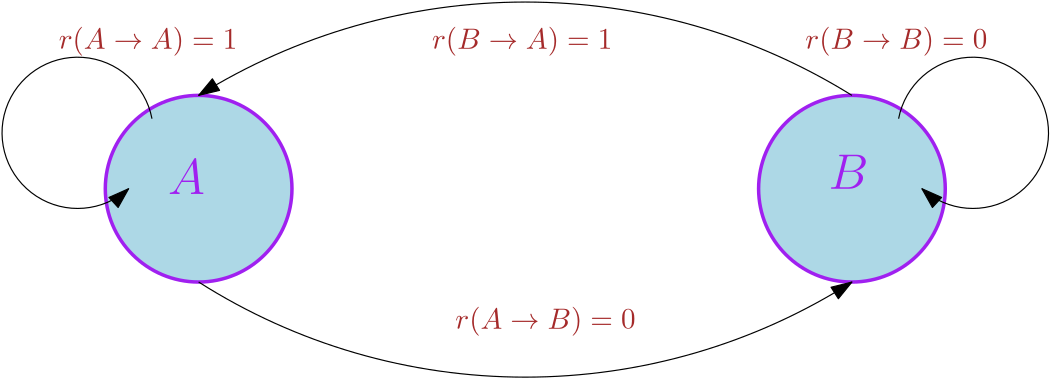
\includegraphics[width=0.6\linewidth]{mdp_2state.png}
  \end{center}
  \vspace{8pt}
In other words, we have $\mathcal{S}=\{A,B\}$, $\mathcal{A}=\{\text{switch}, \text{stay}\}$,
$$
r(A,\text{switch})=0, r(A,\text{stay})=1, r(B,\text{switch})=1, r(B,\text{stay})=0,
$$
$$
P(A|A,\text{switch})=0, P(A|A,\text{stay})=1, P(B|B,\text{switch})=0, P(B|B,\text{stay})=1.
$$
Let $\gamma\in(0,1)$ be the discount factor. Let $\pi_0$ be the policy which always switches states.
  

\begin{questions}
    \question[5]  Compute the value function $\textbf{V}^{\pi_0}$ of $\pi_0$. 
    \question[5]  Compute the optimal value function $\textbf{V}^*$ and optimal policy $\pi^*$.
    \question[5]  Compute $\mathcal{T}\mathbf{V}^{\pi_0}$ where $\mathcal{T}$ is the Bellman optimality operator.
    \question[5]  Compute the greedy policy based on $\textbf{V}^{\pi_0}$. 
    \question[5] Compute the first $5$ updates of Value Iteration algorithm initialized with $\textbf{V}^{\pi_0}$.
    \question[5] Compute the first $5$ updates of Policy Iteration algorithm initialized with $\pi_0$.
\end{questions}

\begin{remark}
What happens if we evaluate the first $10,20,30\dots$ steps of Value Iteration? This example also implies that iterating $n$ times the Bellman optimality operator  is not guaranteed to lead exactly to $\mathbf{V}^*$ for any finite $n \in \mathbb{N}$. 
\end{remark}

Contact: \texttt{nuria.armengolurpi@inf.ethz.ch}

\begin{Solution}
    \begin{enumerate} [label=\alph*)]
        \item
        As the transition is deterministic given the action, we can write
        $$
        \begin{aligned}
        \textbf{V}^{\pi_0}(A) & = \mathbb{E} \left [ \sum_{t=0}^\infty \gamma^t r(s_t, a_t) \mid s_0=A, \pi_0 \right ] \\
        & = r(A, \text{switch}) + \gamma r(B, \text{switch}) + \gamma^2 r(A, \text{switch}) + \gamma^3 r(B, \text{switch}) + \cdots \\
        & = 0 + \gamma + 0 + \gamma^3 + \cdots \\
        & = \gamma \sum_{k=0}^\infty \gamma^{2k} \\
        & = \dfrac{\gamma}{1 - \gamma^2}
        \end{aligned}
        $$
        Note that the last equation holds since we assume $\gamma \in (0,1)$. In like manner,
        $$
        \begin{aligned}
        \textbf{V}^{\pi_0}(B) & = \mathbb{E} \left [ \sum_{t=0}^\infty \gamma^t r(s_t, a_t) \mid s_0=B, \pi_0 \right ] \\
        & = r(B, \text{switch}) + \gamma r(A, \text{switch}) + \gamma^2 r(B, \text{switch}) + \gamma^3 r(A, \text{switch}) + \cdots \\
        & = 1+ 0 + \gamma^2 + 0 + \cdots \\
        & = \sum_{k=0}^\infty \gamma^{2k} \\
        & = \dfrac{1}{1 - \gamma^2}
        \end{aligned}
        $$
        \item
        As the reward for entering $A$ is $1$, the reward for entering $B$ is $0$, and the transition is deterministic, the policy that attains the largest reward would be ``stay at $A$ if the current state is $A$'' and ``switch to $A$ if the current state is $B$'', i.e.
        $$
        \pi^*(A) = \text{stay}
        $$
        $$
        \pi^*(B) = \text{switch}
        $$
        Therefore, the corresponding optimal value function $\textbf{V}^*$ satisfies
        $$
        \begin{aligned}
        \textbf{V}^*(A) & = \mathbb{E} \left [ \sum_{t=0}^\infty \gamma^t r(s_t, a_t) \mid s_0=A, \pi^* \right ] \\
        & = \sum_{t=0}^\infty \gamma^t r(A, \text{stay}) \\
        & = \sum_{t=0}^\infty \gamma^t \\
        & = \dfrac{1}{1 - \gamma}
        \end{aligned}
        $$
        And
        $$
        \begin{aligned}
        \textbf{V}^*(B) & = \mathbb{E} \left [ \sum_{t=0}^\infty \gamma^t r(s_t, a_t) \mid s_0=B, \pi^* \right ] \\
        & = r(B, \text{switch}) + \sum_{t=1}^\infty \gamma^t r(A, \text{stay}) \\
        & = \sum_{t=0}^\infty \gamma^t \\
        & = \dfrac{1}{1 - \gamma}
        \end{aligned}
        $$
        \item
        $$
        \begin{aligned}
        (\mathcal{T}\mathbf{V}^{\pi_0})(A) & = \max_{a \in \mathcal{A}} \left [ r(A, a) + \gamma \sum_{s' \in \mathcal{S}} P(s' \mid A, a) \mathbf{V}^{\pi_0}(s') \right ] \\
        & = \max \{r(A, \text{stay}) + \gamma \mathbf{V}^{\pi_0}(A), r(A, \text{switch}) + \gamma \mathbf{V}^{\pi_0}(B)\} \\
        & = \max \{1 + \dfrac{\gamma^2}{1 - \gamma^2}, 0 + \dfrac{\gamma}{1 - \gamma^2}\} \\
        & = \dfrac{1}{1 - \gamma^2}
        \end{aligned}
        $$
        And
        $$
        \begin{aligned}
        (\mathcal{T}\mathbf{V}^{\pi_0})(B) & = \max_{a \in \mathcal{A}} \left [ r(B, a) + \gamma \sum_{s' \in \mathcal{S}} P(s' \mid B, a) \mathbf{V}^{\pi_0}(s') \right ] \\
        & = \max \{r(B, \text{stay}) + \gamma \mathbf{V}^{\pi_0}(B), r(B, \text{switch}) + \gamma \mathbf{V}^{\pi_0}(A)\} \\
        & = \max \{0 + \dfrac{\gamma}{1 - \gamma^2}, 1 + \dfrac{\gamma^2}{1 - \gamma^2}\} \\
        & = \dfrac{1}{1 - \gamma^2}
        \end{aligned}
        $$
        \item
        The greedy policy picks the action that maximizes $\mathcal{T}\mathbf{V}^{\pi_0}$, i.e. we look for the maximizer of the last question
        $$
        \begin{aligned}
        \pi_1(A) & = \argmax_{a \in \mathcal{A}} \left [ r(A, a) + \gamma \sum_{s' \in \mathcal{S}} P(s' \mid A, a) \mathbf{V}^{\pi_0}(s') \right ] \\
        & = \text{stay}
        \end{aligned}
        $$
        And
        $$
        \begin{aligned}
        \pi_1(B) & = \argmax_{a \in \mathcal{A}} \left [ r(B, a) + \gamma \sum_{s' \in \mathcal{S}} P(s' \mid B, a) \mathbf{V}^{\pi_0}(s') \right ] \\
        & = \text{switch}
        \end{aligned}
        $$
        \item
        Let $\mathbf{V}_0 := \mathbf{V}^{\pi_0}$, we have
        $$
        \mathbf{V}_0(A) = \dfrac{\gamma}{1 - \gamma^2}, \quad \mathbf{V}_0(B) = \dfrac{1}{1 - \gamma^2}
        $$
        $$
        \mathbf{V}_1(A) = (\mathcal{T}\mathbf{V}_0)(A) = \mathbf{V}_1(B) = (\mathcal{T}\mathbf{V}_0)(B) = \dfrac{1}{1 - \gamma^2}
        $$
        $$
        \mathbf{V}_2(A) = (\mathcal{T}\mathbf{V}_1)(A) = \mathbf{V}_2(B) = (\mathcal{T}\mathbf{V}_1)(B) = \dfrac{1 +\gamma - \gamma^2}{1 - \gamma^2}
        $$
        $$
        \mathbf{V}_3(A) = (\mathcal{T}\mathbf{V}_2)(A) = \mathbf{V}_3(B) = (\mathcal{T}\mathbf{V}_2)(B) = \dfrac{1 + \gamma - \gamma^3}{1 - \gamma^2}
        $$
        $$
        \mathbf{V}_4(A) = (\mathcal{T}\mathbf{V}_3)(A) = \mathbf{V}_4(B) = (\mathcal{T}\mathbf{V}_3)(B) = \dfrac{1 + \gamma - \gamma^4}{1 - \gamma^2}
        $$
        $$
        \mathbf{V}_5(A) = (\mathcal{T}\mathbf{V}_4)(A) = \mathbf{V}_5(B) = (\mathcal{T}\mathbf{V}_4)(B) = \dfrac{1 + \gamma - \gamma^5}{1 - \gamma^2}
        $$
        \item
        Note that the algorithm converges from the second step. Policy $\pi_1$ follows question d) and its evaluation follows question b), as $\pi_1$ coincides with the optimal policy $\pi^*$.
        $$
        \pi_0(A) = \text{switch}, \quad \pi_0(B) = \text{switch}
        $$
        $$
        \textbf{V}^{\pi_0}(A) = \dfrac{\gamma}{1 - \gamma^2}, \quad \textbf{V}^{\pi_0}(B) = \dfrac{1}{1 - \gamma^2}
        $$
        $$
        \pi_1(A) = \text{stay}, \quad \pi_1(B) = \text{switch}
        $$
        $$
        \textbf{V}^{\pi_1}(A) = \dfrac{1}{1 - \gamma}, \quad \textbf{V}^{\pi_1}(B) = \dfrac{1}{1 - \gamma}
        $$
        $$
        \pi_2(A) = \text{stay}, \quad \pi_2(B) = \text{switch}
        $$
        $$
        \textbf{V}^{\pi_2}(A) = \dfrac{1}{1 - \gamma}, \quad \textbf{V}^{\pi_2}(B) = \dfrac{1}{1 - \gamma}
        $$
        $$
        \pi_3(A) = \text{stay}, \quad \pi_3(B) = \text{switch}
        $$
        $$
        \textbf{V}^{\pi_3}(A) = \dfrac{1}{1 - \gamma}, \quad \textbf{V}^{\pi_3}(B) = \dfrac{1}{1 - \gamma}
        $$
        $$
        \pi_4(A) = \text{stay}, \quad \pi_4(B) = \text{switch}
        $$
        $$
        \textbf{V}^{\pi_4}(A) = \dfrac{1}{1 - \gamma}, \quad \textbf{V}^{\pi_4}(B) = \dfrac{1}{1 - \gamma}
        $$
        $$
        \pi_5(A) = \text{stay}, \quad \pi_5(B) = \text{switch}
        $$
        $$
        \textbf{V}^{\pi_5}(A) = \dfrac{1}{1 - \gamma}, \quad \textbf{V}^{\pi_5}(B) = \dfrac{1}{1 - \gamma}
        $$
    \end{enumerate}

\end{Solution}

\newpage
%==========================================================================================================
\section{Convergence of Policy Iteration (15 points)}
Consider the policy iteration algorithm for infinite horizon MDPs with a discount factor $\gamma < 1$. Let $\pi_t$ and $\pi_{t+1}$ be the respective policies at time steps $t$ and $t+1$, where $\pi_{t+1}$ is the greedy policy based on the value function $\mathbf{V}^{\pi_t}$.   
From the above example (see Exercise 1), one can observe that the Bellman optimality operator applied to $V^{\pi_t}$ does not in general yield $\mathbf{V}^{\pi_{t+1}}$, i.e., $\mathcal{T}\mathbf{V}^{\pi_t} \neq \mathbf{V}^{\pi_{t+1}}$. \\


In slide 39/53 of Lecture 2, there is a typo:
    \begin{align}
    \| \mathbf{V}^{\pi_{t+1}} - \mathbf{V}^*\|_\infty {\color{red}=} \|\mathcal{T}\mathbf{V}^{\pi_{t}} - \mathcal{T}\mathbf{V}^*\|_\infty 
    \end{align}
This should instead be 
    \begin{align}
    \| \mathbf{V}^{\pi_{t+1}} - \mathbf{V}^*\|_\infty {\color{red}\leq} \|\mathcal{T}\mathbf{V}^{\pi_{t}} - \mathcal{T}\mathbf{V}^*\|_\infty 
    \end{align}
    
Here we aim to prove the linear convergence of policy iteration in a precise manner. 
\begin{questions}
    \question[5] Prove 
    \begin{align*}
	    \mathcal{T} \mathbf{V}^{\pi_{t}}(s) \geq \mathbf{V}^{\pi_t}(s) \quad \quad \forall s \in \mathcal{S}.
    \end{align*} 
 
	\question[5] Prove
     \begin{align*}
	     \mathbf{V}^{\pi_{t+1}}(s) \geq \mathcal{T} \mathbf{V}^{\pi_{t}}(s) \quad \quad \forall s \in \mathcal{S}.
    \end{align*}
    
    \question[5] Using the above, prove the linear convergence of the policy iteration algorithm.
\end{questions}

Contact: \texttt{daniel.paleka@math.ethz.ch}


\begin{Solution}
    \begin{enumerate} [label=\alph*)]
        \item
        We consider only stationary and deterministic policy in the following arguments. 
        $$
        \begin{aligned}
        (\mathcal{T}\mathbf{V}^{\pi_t})(s) & = \max_{a \in \mathcal{A}} \left [ r(s, a) + \gamma \sum_{s' \in \mathcal{S}}P(s' \mid s,a) \mathbf{V}^{\pi_t}(s') \right ] \\
        & = \max_{a \in \mathcal{A}} \mathbf{Q}^{\pi_t}(s, a) \\
        & = \mathbf{Q}^{\pi_t}(s, \pi_{t+1}(s)) \\
        & \geq \mathbf{Q}^{\pi_t}(s, \pi_t(s)) \\
        & = (\mathcal{T}^{\pi_t}\mathbf{V}^{\pi_t})(s) \\
        & = \mathbf{V}^{\pi_t}(s)
        \end{aligned}
        $$
        Or more concisely, which is meanwhile also applicable to the stochastic setting
        $$
        \mathcal{T}\mathbf{V}^{\pi_t} = \mathcal{T}^{\pi_{t+1}}\mathbf{V}^{\pi_t} \geq \mathcal{T}^{\pi_{t}}\mathbf{V}^{\pi_t} = \mathbf{V}^{\pi_t} \\
        $$
        \item
        $$
        \begin{aligned}
        (\mathcal{T}\mathbf{V}^{\pi_t})(s) & = \max_{a \in \mathcal{A}} \mathbf{Q}^{\pi_t}(s, a) \\
        & = \mathbf{Q}^{\pi_t}(s, \pi_{t+1}(s)) \\
        & = r(s, \pi_{t+1}(s)) + \gamma \mathbf{V}^{\pi_t}(s') \\
        & \leq r(s, \pi_{t+1}(s)) + \gamma \mathbf{Q}^{\pi_t}(s', \pi_{t+1}(s')) \\
        & \leq r(s, \pi_{t+1}(s)) + \gamma r(s', \pi_{t+1}(s')) + \gamma^2 \mathbf{Q}^{\pi_t}(s'', \pi_{t+1}(s'')) \\
        & \leq r(s, \pi_{t+1}(s)) + \gamma r(s', \pi_{t+1}(s') + \gamma^2 r(s'', \pi_{t+1}(s'')) + \cdots \\
        & = \mathbf{V}^{\pi_{t+1}}(s)
        \end{aligned}
        $$
        Or more concisely, which is meanwhile also applicable to the stochastic setting
        $$
        \mathcal{T}\mathbf{V}^{\pi_t} = \mathcal{T}^{\pi_{t+1}}\mathbf{V}^{\pi_t} \leq  (\mathcal{T}^{\pi_{t+1}})^2\mathbf{V}^{\pi_t} \leq \cdots \leq \mathbf{V}^{\pi_{t+1}}
        $$
        \item
        From questions a) and b), we have
        $$
        \mathbf{V}^{\pi_{t+1}} \geq \mathcal{T}\mathbf{V}^{\pi_t} \geq \mathbf{V}^{\pi_{t}}
        $$
        This shows that during policy iteration, the value function associated with the corresponding policy is monotonically increasing. Applying the contraction property of the Bellman optimality operator $\mathcal{T}$, i.e.
        $$
        \|\mathcal{T}\mathbf{V}' - \mathcal{T}\mathbf{V}\|_\infty \leq \gamma \|\mathbf{V}' - \mathbf{V} \|_\infty
        $$
        and following the proof on slide 39/53 of Lecture 2, we have
        $$
        \begin{aligned}
        \| \mathbf{V}^{\pi_{t}} - \mathbf{V}^*\|_\infty & \leq \|\mathcal{T}\mathbf{V}^{\pi_{t-1}} - \mathcal{T}\mathbf{V}^*\|_\infty \\
        & \leq \gamma \| \mathbf{V}^{\pi_{t-1}} - \mathbf{V}^*\|_\infty \\
        & \leq \cdots \\
        & \leq \gamma^t \| \mathbf{V}^{\pi_{0}} - \mathbf{V}^*\|_\infty \\
        \end{aligned}
        $$
    \end{enumerate}
\end{Solution}


%==========================================================================================================
\newpage
\section{Bounding Suboptimality via Bellman Error (35 points)}
Consider a tabular MDP with finite state space $\mathcal{S}$ and action space $\A$. 
\begin{questions}

\question[10] 
Recall the Bellman optimality operator $\ST$ and the Bellman expectation operator $\ST^\pi$ from the lecture, defined on the space of value functions.
Formally define analogous operators $\ST_Q$ and $\ST^\pi_Q$ on the space of state-action value Q-functions.


\question[10] For any state-action value functions $\mathbf{Q}, \mathbf{Q}'$, prove:
\begin{align*}
    \abs {\max_{a \in \mathcal{A} } \mathbf{Q}(s,a) - \max_{a \in \mathcal{A} }\mathbf{Q}'(s,a)} \le \norm{\mathbf{Q} - \mathbf{Q}'}_\infty \forall s \in \mathcal{S}.
\end{align*}
Show both defined operators are $\gamma$-contractions under the $\ell_\infty$-norm.

\question[5]
For any state-action value function $\mathbf{Q}$, prove:
\begin{align*}
    \norm{\mathbf{Q} - \mathbf{Q}^{*}}_\infty \leq  \frac{\norm{\mathbf{Q} - \mathcal{T}_Q \mathbf{Q}}_\infty}{1-\gamma} .
\end{align*}

\question[10] 
 Now we are ready for the main point. Let $Q$ be a state-action value function, and let $\pi$ be the greedy policy with respect to $Q$, that is, $\pi = \argmax_a Q(\cdot, a)$ .
 Show that the value function  $V^\pi$ for this policy satisfies
\begin{align*}
   \norm{\mathbf{V}^{\pi} - \mathbf{V}^{*}}_\infty \leq \frac{2\norm{\mathbf{Q} - \mathcal{T}_Q\mathbf{Q}}_\infty}{1-\gamma}.
\end{align*}

where $\mathcal{T}_Q$ is the Bellman optimality operator on the space of state-action value Q-functions.
\end{questions}

Contact: \texttt{nuria.armengolurpi@inf.ethz.ch}

\begin{Solution}
    \begin{enumerate} [label=\alph*)]
        \item
        Referring to the Bellman optimality and expectation operator, we analogously define
        $$
        (\ST_Q \mathbf{Q})(s,a) := r(s,a) + \gamma \left [ \sum_{s' \in \mathcal{S}} P(s' \mid s, a) \left (\max_{a' \in \mathcal{A}} \mathbf{Q}(s', a') \right ) \right ]
        $$
        $$
        (\ST_Q^{\pi} \mathbf{Q})(s,a) := r(s,a) + \gamma \left [ \sum_{s' \in \mathcal{S}} P(s' \mid s, a) \left (\sum_{a' \in \mathcal{A}} \pi(a' \mid s') \mathbf{Q}(s', a') \right ) \right ]
        $$
        \item
        Note that
        $$
        \begin{aligned}
        \mathbf{Q}(s,a) - \mathbf{Q}'(s,a) & \leq \abs{\mathbf{Q}(s,a) - \mathbf{Q}'(s,a)} , \quad \forall s \in \mathcal{S} \\
        \mathbf{Q}(s,a) & \leq \abs{\mathbf{Q}(s,a) - \mathbf{Q}'(s,a)} + \mathbf{Q}'(s,a) \\
        \max_{a \in \mathcal{A} } \mathbf{Q}(s,a) & \leq \max_{a \in \mathcal{A} } \abs{\mathbf{Q}(s,a) - \mathbf{Q}'(s,a)} + \max_{a \in \mathcal{A} } \mathbf{Q}'(s,a) \\
        \end{aligned}
        $$
        Therefore, we have
        $$
        \abs {\max_{a \in \mathcal{A} } \mathbf{Q}(s,a) - \max_{a \in \mathcal{A} }\mathbf{Q}'(s,a)} \le \max_{a \in \mathcal{A}} \abs{\mathbf{Q}(s,a) - \mathbf{Q}'(s,a)} = \norm{\mathbf{Q} - \mathbf{Q}'}_\infty, \quad \forall s \in \mathcal{S}
        $$
        To show contraction property of $\ST_Q$ and $\ST_Q^{\pi}$, observe
        $$
        \begin{aligned}
        \|\ST_Q \mathbf{Q} - \ST_Q\mathbf{Q}'\|_\infty & = \max_{s \in \mathcal{S}} \gamma \left [ \sum_{s' \in \mathcal{S}} P(s' \mid s, a) \abs{\max_{a' \in \mathcal{A}} \mathbf{Q}(s', a') - \max_{a' \in \mathcal{A}} \mathbf{Q}'(s', a') } \right ] \\
        & \leq \max_{s \in \mathcal{S}} \gamma \left [ \sum_{s' \in \mathcal{S}} P(s' \mid s, a) \norm{\mathbf{Q} - \mathbf{Q}'}_\infty \right ] \\
        & = \gamma \norm{\mathbf{Q} - \mathbf{Q}'}_\infty
        \end{aligned}
        $$
        Similarly,
        $$
        \begin{aligned}
        \|\ST_Q^{\pi} \mathbf{Q} - \ST_Q^{\pi}\mathbf{Q}'\|_\infty & = \max_{s \in \mathcal{S}} \gamma \left [ \sum_{s' \in \mathcal{S}} P(s' \mid s, a) \left (\sum_{a' \in \mathcal{A}} \pi(a' \mid s') \abs{\mathbf{Q}(s', a') - \mathbf{Q}'(s', a')} \right ) \right ] \\
        & \leq \max_{s \in \mathcal{S}} \gamma \left [ \sum_{s' \in \mathcal{S}} P(s' \mid s, a) \left (\sum_{a' \in \mathcal{A}} \pi(a' \mid s') \max_{a' \in \mathcal{A}} \abs{\mathbf{Q}(s', a') - \mathbf{Q}'(s', a')} \right ) \right ] \\
        & \leq \max_{s \in \mathcal{S}} \gamma \left [ \sum_{s' \in \mathcal{S}} P(s' \mid s, a) \sum_{a' \in \mathcal{A}} \pi(a' \mid s') \norm{\mathbf{Q} - \mathbf{Q}'}_\infty \right ] \\
        & = \gamma \norm{\mathbf{Q} - \mathbf{Q}'}_\infty
        \end{aligned}
        $$
        \item
        Note that $\mathbf{Q}^{\pi}$ is a fixed point of $\ST_Q^{\pi}$, i.e. $\mathbf{Q}^{\pi} = \ST_Q^{\pi} \mathbf{Q}^{\pi}$. Using the conclusion from question b) and the triangle inequality of infinity norm, we can write
        $$
        \norm{\mathbf{Q} - \mathbf{Q}^{\pi}}_\infty \leq \norm{\mathbf{Q} - \ST_Q^{\pi} \mathbf{Q}}_\infty + \norm{\ST_Q^{\pi} \mathbf{Q} - \mathbf{Q}^{\pi}}_\infty \leq \norm{\mathbf{Q} - \ST_Q^{\pi} \mathbf{Q}}_\infty + \gamma \norm{\mathbf{Q} - \mathbf{Q}^{\pi}}_\infty
        $$
        from which it follows that
        $$
        \norm{\mathbf{Q} - \mathbf{Q}^{\pi}}_\infty \leq  \frac{\norm{\mathbf{Q} - \mathcal{T}_Q^\pi \mathbf{Q}}_\infty}{1-\gamma}
        $$
        Similarly, note that $\mathbf{Q}^{*}$ is a fixed point of $\ST_Q$, we have
        $$
        \norm{\mathbf{Q} - \mathbf{Q}^{*}}_\infty \leq \norm{\mathbf{Q} - \ST_Q \mathbf{Q}}_\infty + \norm{\ST_Q \mathbf{Q} - \mathbf{Q}^{*}}_\infty \leq \norm{\mathbf{Q} - \ST_Q \mathbf{Q}}_\infty + \gamma \norm{\mathbf{Q} - \mathbf{Q}^{*}}_\infty
        $$
        which is equivalent to the original inequality
        $$
        \norm{\mathbf{Q} - \mathbf{Q}^{*}}_\infty \leq  \frac{\norm{\mathbf{Q} - \mathcal{T}_Q \mathbf{Q}}_\infty}{1-\gamma}
        $$
        noting that $\gamma \in (0,1)$.
        \item
        Since $\pi$ is a greedy policy with respect to $\mathbf{Q}$, it holds that
        $$
        \mathbf{V}^\pi = \mathbf{Q}^\pi(s,\pi(s)) = \max_{a \in \mathcal{A}} \mathbf{Q}^\pi(s,a), \quad \ST_Q^\pi \mathbf{Q} = \ST_Q \mathbf{Q}
        $$
        Also note by optimality conditions
        $$
        \mathbf{V}^* = \mathbf{Q}^*(s,\pi^*(s)) = \max_{a \in \mathcal{A}} \mathbf{Q}^*(s,a)
        $$
        By the triangle inequality of the infinity norm and using the result from question b), we have
        $$
        \begin{aligned}
        \norm{\mathbf{V}^{\pi} - \mathbf{V}^{*}}_\infty & \leq \norm{\mathbf{V} - \mathbf{V}^\pi}_\infty + \norm{\mathbf{V} - \mathbf{V}^{*}}_\infty \\
        & = \max_{s \in \mathcal{S}} \abs{\max_{a \in \mathcal{A}} \mathbf{Q}(s,a) - \max_{a \in \mathcal{A}} \mathbf{Q}^\pi(s,a)} + \max_{s \in \mathcal{S}} \abs{\max_{a \in \mathcal{A}} \mathbf{Q}(s,a) - \max_{a \in \mathcal{A}} \mathbf{Q}^*(s,a)} \\
        & \leq \norm{\mathbf{Q} - \mathbf{Q}^\pi}_\infty + \norm{\mathbf{Q} - \mathbf{Q}^{*}}_\infty
        \end{aligned}
        $$
        Using the two inequalities derived in question c), we write
        $$
        \norm{\mathbf{V}^{\pi} - \mathbf{V}^{*}}_\infty \leq \norm{\mathbf{Q} - \mathbf{Q}^\pi}_\infty + \norm{\mathbf{Q} - \mathbf{Q}^{*}}_\infty \leq \frac{\norm{\mathbf{Q} - \mathcal{T}_Q^\pi \mathbf{Q}}_\infty}{1-\gamma} + \frac{\norm{\mathbf{Q} - \mathcal{T}_Q \mathbf{Q}}_\infty}{1-\gamma} = \frac{2 \norm{\mathbf{Q} - \mathcal{T}_Q \mathbf{Q}}_\infty}{1-\gamma}
        $$
    \end{enumerate}
\end{Solution}


\clearpage
%==========================================================================================================




\section{Reading: The Value Function Polytope (20 points)}
In the reading exercise, you are expected to read some material and write a paragraph for each question.
The questions may not be well-posed, and are intended to encourage reading and thinking;
the grading here will be more lenient than in the previous problems.

In~\cite{dadashi2019value} the authors characterize the geometry of the space of all possible value functions given a Markov Decision Process. Then, they illustrate the dynamics of RL algorithms in the value function space, including value iteration, policy iteration, policy gradient methods, etc. Read the paper \cite{dadashi2019value} and think about the following questions. \footnote{Extending \cite{dadashi2019value} by investigating the interplay between non-convexity and dynamics
may be a nice idea for the course project.}

\begin{questions}
\question[5]
On the first page, Figure 1 shows a convex space of policies mapped into a non-convex space of value functions.
Why does this happen, philosophically? (You can think of your explanation, as we do not have one single correct answer.)


\question[5]
In Theorem 1, the authors consider the set of policies that differ only in one state $s$. Why is it necessary that policies differ only in a single state?
What happens if we interpolate between two policies that differ in more states instead of only in a single one? (Answer in simple heuristic terms, no proofs needed.)\\

Hint: look at Lemma 3.

\question[10] 
What is your take-away from this paper? What is the main limitation of the paper? 
\end{questions}

Contact: \texttt{daniel.paleka@math.ethz.ch}


\begin{Solution}
\begin{enumerate} [label=\alph*)]
        \item
        Under a convex policy space $\mathcal{P}(\mathcal{A})^\mathcal{S}$ setting, a convex combination of two valid policies $\pi_1$ and $\pi_2$ remains valid, i.e. $\pi' = \alpha \pi_1 + (1-\alpha) \pi_2 \in \mathcal{P}(\mathcal{A})^\mathcal{S}, \forall \alpha \in [0, 1]$. However the corresponding value function vector $V^{\pi'}$ does not necessarily coincide with the convex combination of $V^{\pi_1}$ and $V^{\pi_2}$, as the mapping functional $f_v: \mathcal{P}(\mathcal{A})^\mathcal{S} \rightarrow \mathbb{R}^\mathcal{S}$ has fundamental non-linearity which can be far more complex than being an affine transformation. Moreover, with different sets of states being fixed and freed when varing the policies, $V^{\pi_1}$ and $V^{\pi_2}$ live on their own induced space of value function respectively. By Corollary 1, they can be expressed as a convex combination by value functions of their own $\{s_1, \ldots, s_k\}$-deterministic policies respectively. However, the convex combination of value functions from two different induced subspaces is rather meaningless. As example 1 shows, the paths traced by interpolating between two arbitrary policies may be neither linear, nor monotonic. 
        
        As the paper points out, this can happen when value functions along two different line segments cross. At that intersection, there are two policies with the same value function but that do not agree on either state. This is especially the case when the environment of the Markov Decision Process is highly symmetric, or when there exist two distinct but equally beneficial actions at most states. 
        
        Under the Markov Decision Process setting, it is well interpreted that the space of value function $\mathcal{V}$ is bounded and flat-edged as shown in the paper. With the arguments above being listed, it makes no sense to require $\mathcal{V}$ convex. 
        
        \item
        It is necessary that policies differ only in a single dimension because the paper intends to present the line theorem, whose characterization forms the basis to prove the other two results, including the relationship between faces and semi-deterministic policies and its generalization to higher dimensions. In their sub-polytope characterization it is demonstrated that varying a policy along $d$ states generates a $d$ dimensional sub-polytope. These results are based on the line theorem which provides guarantees of monotonic improvement as well as a line-like variation in the space of value functions. To argue for a general claim, it is always helpful to start from the most special and simplest case.
        
        If we interpolate between two policies that differ in $k$ states instead of only in a single one, Lemma 3 shows that the induced space of value function loses at least $k$ degrees of freedom, specifically that it lies in a $|\mathcal{S}| - k$ dimensional affine vector space. As a more general conclusion, Lemma 3 in turn explains the line theorem, i.e., for $k = |\mathcal{S}| - 1$, the value functions lie on a line.
        
        \item
        \textbf{Take-away}
        
        My take-away of the paper is based on its contribution in two focuses.
        
        In the section of the characterization of the nature of the space of value functions in finite state action Markov Decision Processes, I understood how to relate its geometric and topological properties to the properties of the corresponding policies that induce the space. It is surprising that the line theorem shows that the value functions of all policies agreed on all but state $s$ are bounded by two $s$-deterministic policies and furthermore, that one can generate the set of value functions by tracking either the convex combination of two value functions mapped by the two bounding policies or the mapped value function from the convex combination of the two policies. The line theorem provides guarantees of monotonic improvement as well as a line-like variation in the space of value functions. With it being illustrated, it is natural to extend it to the case when we fix the policies on $k$ states instead of only one. Moreover, convex mixtures of policies can describe curves which is non-linear in the mixing weights, which shows that the paths traced by interpolating between two arbitrary policies may be neither linear, nor monotonic. Finally, I understood that the boundary of the space of value functions is a subset of the ensemble of value functions of semi-deterministic policies. Besides these conclusions, I also learnt how to express a clear flow of thoughts in writing the paper - first start with a simple example with illustrations to prove some conclusion in a special context, then extend it to a more general setting based on the previous results. 
        
        In the section of dynamics in the value polytope I understood the visualized expected behaviour and pitfalls of common algorithms. Specifically, value iteration generates a sequence of value functions that may not map to any policy. The sequence of value functions visited by policy iteration corresponds to value functions of deterministic policies. The convergence rate of policy gradient strongly depends on the initial condition and the convergence might fall into sub-optimal solutions. Potential solutions include regularization with entropy, which encourages policies to move away from the boundary of the polytope, and natural policy gradient, which is  less prone to accumulation as a result of better conditioned step-size. Besides these conclusions, I also learnt how to illustrate experiments results in a clear and efficient fashion, being informative and concise at the same time.
        
        \vspace{1em}
        \textbf{Limitation}
        
        The presentation of the study outcome is very clear as the paper visualizes the results in a well-organized way. However, one fundamental limit can be the generalization of the conclusions to higher dimensions, in particular in the second section where it focuses on analyzing the dynamics of common algorithms in the value function polytope. It is not yet discussed if the conclusions hold well in Markov Decision Processes with much more complex state and action spaces. Moreover, a high dimensional setting may cause problems as the computational cost increases exponentially with dimensions of both states and actions.
        
        Also, as the paper points out, although those geometric concepts make sense for finite state action spaces, it is not clear how they generalize to the continuous case.
        
        Finally, the paper assumes a perfect knowledge of the model of environment - in this case they can compute the value function precisely. However, in a more general model-free reinforcement learning context, the sampling based applications of the algorithms studied may not be able to deliver a precise estimation of value functions.
        
\end{enumerate}
\end{Solution}



\clearpage
\section{Bonus: Convergence of Inexact Policy Iteration (10 points)}
Consider a tabular MDP with finite state space $\mathcal{S}$ and action space $\mathcal{A}$ and discount factor $\gamma$. In Exercise 2, we proved the linear convergence of the policy iteration algorithm. \\

Now consider the ``inexact'' version of the policy iteration algorithm, i.e., in each step we compute a function $\mathbf{V}_t$ such that
\begin{align*}
    \max_{s \in \mathcal{S}} | \mathbf{V}_t(s) - \mathbf{V}^{\pi_t}(s) | \le \epsilon
\end{align*}
for all steps $t \ge 0$ and some $\epsilon > 0$. Then the algorithm sets $\pi_{t+1}$ to the greedy policy with respect to $\mathbf{V}_t$. We can interpret $\epsilon$ as an error incurred during the policy evaluation step, as for example errors due to simulation. 

 Show that the sequence of policies $\pi_t$ generated by this algorithm satisfies:
\begin{align*}
    \limsup_{t \rightarrow \infty} \max_{s \in \mathcal{S}}  |\mathbf{V}^{\pi_t}(s) - \mathbf{V}^*(s)| \le \frac{2 \gamma \epsilon}{(1 - \gamma)^2}.
\end{align*}

Contact: \texttt{daniel.paleka@math.ethz.ch}


\begin{Solution}
Consider the maximum error bound of the inexact policy iteration algorithm
$$
\max_{s \in \mathcal{S}} | \mathbf{V}_t(s) - \mathbf{V}^{\pi_t}(s) | \le \epsilon, \quad \text{i.e.} \quad \|\mathbf{V}_t - \mathbf{V}^{\pi_t}\|_\infty \leq \epsilon
$$
we have
\begin{equation} \label{(5.1)}
    \mathbf{V}^{\pi_t} + \epsilon \textbf{e} \geq \mathbf{V}_t
\end{equation}
\begin{equation} \label{(5.2)}
    \mathbf{V}_t \geq \mathbf{V}^{\pi_t} - \epsilon \textbf{e}
\end{equation}
where $\textbf{e}$ represents the all-ones vector in state space $\mathcal{S}$.
Apply $\ST^{\pi_{t+1}}$ to both sides of inequality (\ref{(5.1)}) and $\ST$ to both sides of inequality (\ref{(5.2)}). By the monotonicity of Bellman operator, we obtain
\begin{equation} \label{(5.3)}
    \ST^{\pi_{t+1}} \mathbf{V}^{\pi_t} + \gamma \epsilon \textbf{e} \geq \ST^{\pi_{t+1}} \mathbf{V}_t = \ST \mathbf{V}_t
\end{equation}
\begin{equation} \label{(5.4)}
    \ST \mathbf{V}_t \geq \ST \mathbf{V}^{\pi_t} - \gamma \epsilon \textbf{e}
\end{equation}
Combining inequalities (\ref{(5.3)}) and (\ref{(5.4)}), we get
\begin{equation} \label{(5.5)}
    \ST \mathbf{V}^{\pi_t} \leq \ST^{\pi_{t+1}} \mathbf{V}^{\pi_t} + 2 \gamma \epsilon \textbf{e}
\end{equation}
Note that $\mathbf{V}^{\pi_t} = \ST^{\pi_t} \mathbf{V}^{\pi_t} \leq \ST \mathbf{V}^{\pi_t}$, we further have
\begin{equation} \label{(5.6)}
    \mathbf{V}^{\pi_t} \leq \ST^{\pi_{t+1}} \mathbf{V}^{\pi_t} + 2 \gamma \epsilon \textbf{e}
\end{equation}

We finish the proof by applying the following Lemma.

\vspace{1em}
\begin{lemma}
For $c \geq 0$ and some $\mathbf{V}$ such that $\mathbf{V} \leq \ST^{\pi} \mathbf{V} + c \mathbf{e}$, we have
$$
\mathbf{V} \leq \mathbf{V}^\pi + \dfrac{c \mathbf{e}}{1 - \gamma}
$$
\end{lemma}

\textit{Proof.} \quad
Note if we iteratively apply $\ST^\pi$, we have
$$
\mathbf{V} \leq \ST^{\pi} \mathbf{V} + c \mathbf{e}
$$
$$
\ST^{\pi} \mathbf{V} \leq (\ST^{\pi})^2 \mathbf{V} + \gamma c \mathbf{e}
$$
$$
\vdots
$$
$$
(\ST^{\pi})^{k-1} \mathbf{V} \leq (\ST^{\pi})^k \mathbf{V} + \gamma^{k-1} c \mathbf{e}
$$
By adding up the both sides, we obtain
$$
\textbf{V} \leq (\ST^\pi)^k \textbf{V} + \sum_{i=0}^{k-1} \gamma^{i} c \textbf{e}
$$
Note that $\lim_{k \rightarrow \infty} (\ST^\pi)^k \textbf{V} = \textbf{V}^\pi$ and $\sum_{i=0}^\infty \gamma^{i} = \dfrac{1}{1-\gamma}$. Letting $k \rightarrow \infty$ gives the desired result. \begin{flushright} $\square$ \end{flushright}

Applying the Lemma to (\ref{(5.6)}), we get
\begin{equation} \label{(5.7)}
    \mathbf{V}^{\pi_t} \leq \mathbf{V}^{\pi_{t+1}} + \frac{2 \gamma \epsilon}{1 - \gamma} \textbf{e}
\end{equation}

Observe
\begin{equation} \label{(5.8)}
\begin{aligned}
    \mathbf{V}^* - \mathbf{V}^{\pi_{t+1}} & = \mathbf{V}^* - \ST^{\pi_{t+1}} \mathbf{V}^{\pi_{t+1}} \\
    & = \mathbf{V}^* - \ST^{\pi_{t+1}} \mathbf{V}^{\pi_{t}} + (\ST^{\pi_{t+1}} \mathbf{V}^{\pi_{t}} - \ST^{\pi_{t+1}} \mathbf{V}^{\pi_{t+1}}) \\
    & \leq \mathbf{V}^* - \ST^{\pi_{t+1}} \mathbf{V}^{\pi_{t}} + \frac{2 \gamma^2 \epsilon}{1 - \gamma} \textbf{e}
\end{aligned}
\end{equation}
where the last inequality follows from the contraction property of Bellman operator and the conclusion of (\ref{(5.7)}). By subtracting $\mathbf{V}^*$ with the both sides of inequality (\ref{(5.5)}), we obtain
\begin{equation} \label{(5.9)}
     \mathbf{V}^* - \ST^{\pi_{t+1}} \mathbf{V}^{\pi_t} - 2 \gamma \epsilon \textbf{e} \leq \mathbf{V}^* - \ST \mathbf{V}^{\pi_t}
\end{equation}
Note that
\begin{equation} \label{(5.10)}
    \mathbf{V}^* - \ST \mathbf{V}^{\pi_t} = \ST \mathbf{V}^* - \ST \mathbf{V}^{\pi_t} \leq \gamma \|\mathbf{V}^* - \mathbf{V}^{\pi_t}\|_\infty
\end{equation}
Together with inequality (\ref{(5.9)}), we derive
\begin{equation} \label{(5.11)}
    \mathbf{V}^* - \ST^{\pi_{t+1}} \mathbf{V}^{\pi_t} \leq \gamma \|\mathbf{V}^* - \mathbf{V}^{\pi_t}\|_\infty + 2 \gamma \epsilon \textbf{e}
\end{equation}
Then substituting inequality (\ref{(5.11)}) back in (\ref{(5.8)}), we get
\begin{equation}
    \mathbf{V}^* - \mathbf{V}^{\pi_{t+1}} \leq (\mathbf{V}^* - \ST^{\pi_{t+1}} \mathbf{V}^{\pi_{t}}) + \frac{2 \gamma^2 \epsilon}{1 - \gamma} \textbf{e} \leq \gamma \|\mathbf{V}^* - \mathbf{V}^{\pi_t}\|_\infty + 2 \gamma \epsilon \textbf{e} + \frac{2 \gamma^2 \epsilon}{1 - \gamma} \textbf{e}
\end{equation}
which is equivalent to
\begin{equation}
    \|\mathbf{V}^* - \mathbf{V}^{\pi_{t+1}}\|_\infty \leq \gamma \|\mathbf{V}^* - \mathbf{V}^{\pi_t}\|_\infty + \frac{2 \gamma \epsilon}{1 - \gamma}
\end{equation}
Let
$$
\zeta := \limsup_{t \rightarrow \infty} \max_{s \in \mathcal{S}}  |\mathbf{V}^{\pi_t}(s) - \mathbf{V}^*(s)| = \limsup_{t \rightarrow \infty} \|\mathbf{V}^{\pi_t} - \mathbf{V}^*\|_\infty
$$
we can write
$$
\zeta \leq \gamma \zeta + \frac{2 \gamma \epsilon}{1 - \gamma}
$$
which yields the desired result \footnote{Some ideas in the proof workflow above come from \cite{ie3186}.}
$$
\zeta = \limsup_{t \rightarrow \infty} \max_{s \in \mathcal{S}}  |\mathbf{V}^{\pi_t}(s) - \mathbf{V}^*(s)| \le \frac{2 \gamma \epsilon}{(1 - \gamma)^2}
$$

\end{Solution}


\clearpage

\bibliographystyle{plain}
\bibliography{references}

\end{document}
